\documentclass[11pt]{article}
\usepackage{appendix}
\usepackage{graphicx} 
\usepackage{setspace}
\usepackage{amsmath,float,verbatim,multicol}
\usepackage{array}
\usepackage{lscape}
\usepackage{hyperref}

\usepackage{amssymb}
\bibliographystyle{plainnat}
\usepackage[round]{natbib}
\usepackage{multirow}
\usepackage{xcolor}

\setlength{\textheight}{8.8in} \setlength{\textwidth}{6.3in}
\setlength{\oddsidemargin}{0.2in} \setlength{\topmargin}{-0.30in}
\setlength{\footnotesep}{10.0pt}

\newcommand{\ol}{\overline}



\renewcommand{\baselinestretch}{1.25}
\title{Estimating/Calibrating a Structural Model}
\author{ Trevor Gallen \\ Econ 64200 }
\date{Fall 2022}

\begin{document}
\bibliographystyle{myplainnat}
%\bibpunct{(}{)}{;}{a}{}{,}6868

\maketitle


\textbf{Deliverables}
\begin{itemize}
\item You should have a word/\LaTeX document that has three sections: 
\begin{enumerate}
\item Discusses the model and answers the questions I pose throughout.
\item Contains the tables and figures you will produce.
\item Contains a discussion of your programming choices if you had to make any.
\end{enumerate}
\item You should have a Matlab file or set of files (zipped) that contain \textbf{all} your programs and raw data.  There should be a file called ``Main.M" that produces everything I need in one click.
\end{itemize}
\ \\
\ \\


\section{Model}
Take the model from Homework 2, repeated here for convenience, with slightly different  parts, highlighted in {\color{red}{red}}:
Households have Stone-Geary utility over consumption $c_t$:
$$u(c_t,L_t)=\sqrt(c_t-1)$$
Their income each period is the sum of permanent income $P_t$ and a transitory shock $\epsilon_t$:
$$ Y_t=P_t+\epsilon_t$$
Where:
$$\epsilon_t\sim\mathcal{N}(0,\sigma^2_\epsilon)$$
Permanent income is a random walk:
$$P_t=P_{t-1}+\zeta_t$$
Where:
$$\zeta_t\sim\mathcal{N}(0,\sigma^2_\zeta)$$
Households face the budget constraint:
$$Y_t+(1+r)s_{t-1}=c_t+s_t$$
And the borrowing constraint:  $s_t\geq \overline{s}$.\\

Households maximize the net present value of utility, discounted at a rate $0<{\color{red}{\beta}}<1$. Assume that households live until period $T$.\\

Now, let the following numerical assumptions hold:
\begin{table}[ht!]
\centering
\begin{tabular}{lcc}
\hline
\hline
\multicolumn{3}{c}{Table 1: Calibration}\\
\hline
Concept & Parameter & Value \\ 
Lifespan & T & 45 \\
Discount factor & $\beta$ & \textcolor{red}{???}\\
Borrowing constraint & $\overline{s}$ & -0.2 \\
Initial permanent income:  & $P_0$ & 5\\
Variance of permanent income shock:  & $\sigma^2_\zeta$ & 0.02\\
Variance of transitory income shock:  & $\sigma^2_\epsilon$ & 0.04\\
Interest rates:  & $r_{t}$ & 0.05\\
Initial savings:  & $s_{0}$ & $\sim\mathcal{N}(0,$\textcolor{red}{???})\\
\hline
\hline
\end{tabular}
\caption{Note that $s_0$ is truncated normal at $\overline{s}$}
\end{table}

\textbf{Question 1:}   Your goal is to calibrate this structural model by finding {\textcolor{red}{$\beta$}} and {\textcolor{red}{$\sigma^2_\zeta$}}  such that, in expectation:
$$mean(\log(c_{30}^{sim})/\log(c_{29}^{sim}))=1.001788$$
$$Var((s_2^{sim})))=0.00409$$

To do so, you need to have an estimating ``outer loop" and a value-function solving and simulating ``inner loop."  Homework 2 created a file that 1) solved household models and (2) simulated households \emph{given}  $\beta$ and $\sigma^2_{s_0}$.  Your goal is to now (1) create a ``wrapper" function that \emph{takes}  $\beta$ and $\sigma^2_{s_0}$and spits out (for instance) the squared sum of difference between your simulated result and your target result, and chooses  $\beta$ and $\sigma^2_{s_0}$ to minimize that sum of squared errors.\\
\ \\
This is the core of simulated method of moments/``calibration."  \ \\
\ \\
\textbf{Suggested Solutions}:\\

This homework had a few traps!  Broadly, the goal was to introduce you to how to estimate a structural model via simulated method of moments (our minimum distance estimator.)
\begin{itemize}
\item Write down code to solve for an agent's policy function $g$ as a function of parameters to be estimated $\theta$
\item Simulate agents 
\item Find sum of errors of simulated vs data moments
\item Change $\theta$ until this is minimized (or zero)
\end{itemize}

However, there were a few issues you had to think about:
\begin{itemize}
\item Any errors in your solution (due to a sparse grid for instance) would yield errors in the simulation, and thus in the estimator
\item Any errors in your simulation (due to too-few observations for instance) would yield errors in the simulation's results, and thus in the estimator
\item Massive errors would be caused by not setting a common seed for the random number generator across function calls
\item Any of the above three would cause a derivative-based solver to have a hard time (can't take (accurate) derivatives when your surface is changing).  Derivatives would be all noise, convergence is extremely unlikely.
\item Depending on how you did the simulation, you could end up with a state variable outside the bounds you set up.  This is \emph{particularly} a problem when we're changing the variance of shocks!  Increasing variance 
\item It is possible not to be able to fit a structural model even if you have as many moments as parameters (this was the case here). ( \# moments = \# parameters is not enough!)
\item Flat regions of error as a function of parameters will cause high standard errors (think Fisher Information matrix!)
\end{itemize}

Each iteration took a while, as will happen with a lot of dynamic structural estimation!  To think about why, imagine that you might be iterating many many nested loops!
\begin{itemize}
\item Outermost loop:  search over parameters (estimation)
\item Middle loop: given parameters (outermost loop) \& solutions (inner loop) search to find equilibrium between agents (CGE-style), such as wages clearing markets, or agents beliefs about other agents (Krusell-Smith style)
\item Inner loop:  given parameters (outermost) and wages/equilibrum objects (middle loop), find agent's solution
\end{itemize}
In this case we just had an outermost loop and an inner loop.  I used Matlab's surrogate optimization, but you could have used patternsearch or any of the minimizers.  \emph{However}, derivative-based minimizers were subject to error, as discussed above.\\

When I did, I found:  $\beta=0.8904$, and $\sigma^2_{s_0}= 0.36511$, which isn't too far from the original $\beta=0.9$ that I used to generate the moments, but very far from the  and $\sigma^2_{s_0}= 0.1$.  Why?  Looking at the sampled simulated moment errors with respect to the parameter inputs (see Figure \ref{Moments}, you see that we are very ``flat" around the minimum--$\sigma^2_{s_0}$ doesn't map very well into our moments (they were poorly picked!).  If you think about what the Fisher Information matrix would say about the standard errors implied in Figure \ref{Moments}, you'd see that the second derivative seems very low (with low off-diagonals), so the inverse of that matrix is very large--large standard errors on both.  Put another way, if you had simulated this differently (different seed), you might have gotten almost anywhere on the flat region.  This problem was \emph{not} well-identified, primarily due to the second moment.

\begin{figure}[ht!]
\centering
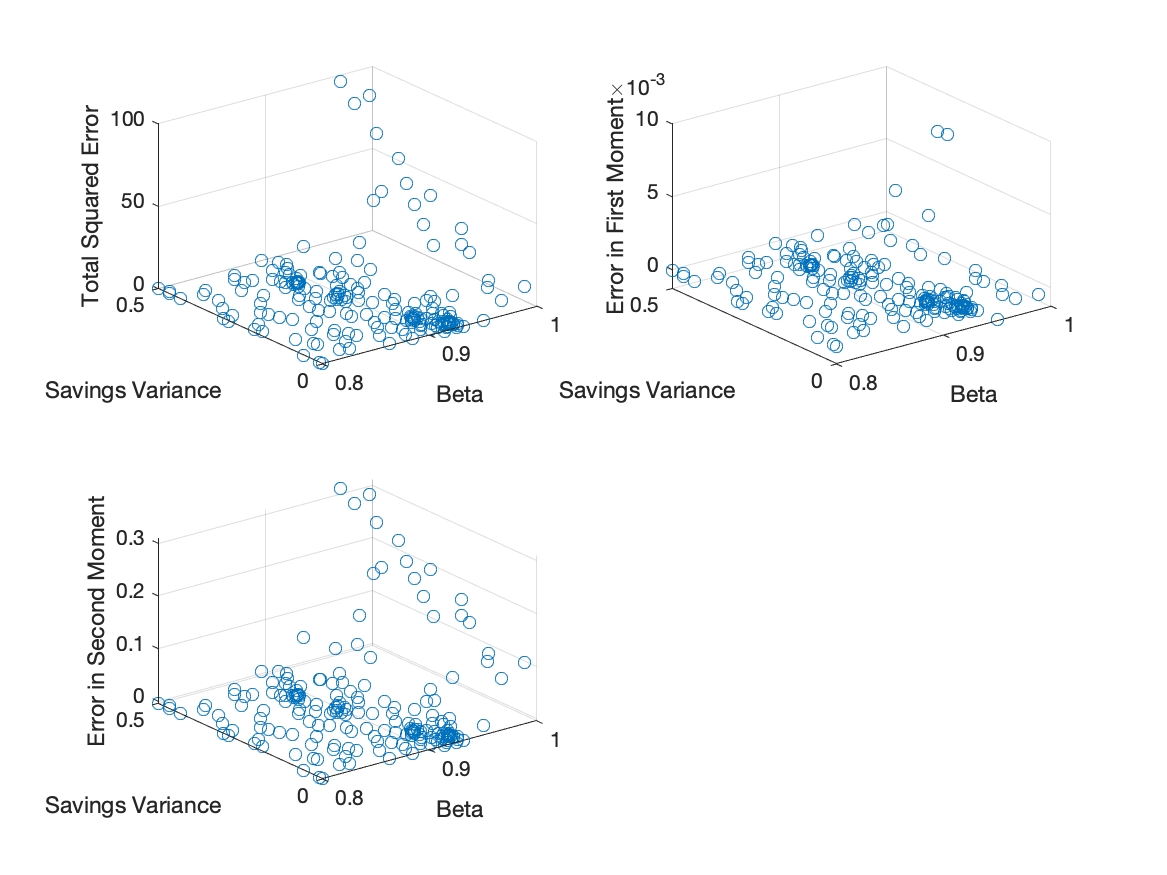
\includegraphics[scale=0.5]{IdentificationFig.png}
\caption{Total squared error, error of moment \#1 (growth) and moment \#2 (savings variance).}
\label{Moments}
\end{figure}

\end{document}





